\chapter{Lattice Paths}
\section{Problem Description}
Starting in the top left corner of a $2 \times 2$ grid, and only being able to move to the right and down, there are exactly
routes to the bottom right corner.

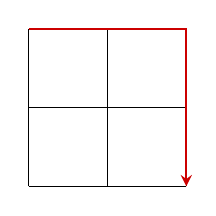
\begin{tikzpicture}
	\draw (0,0) grid (2, -2);
	\draw [->, >=stealth, thick, red!80!black] (0,0) -| (2, -2);
\end{tikzpicture}
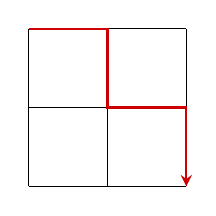
\begin{tikzpicture}
	\draw (0,0) grid (2, -2);
	\draw [->, >=stealth, thick, red!80!black] (0,0) -| (1, -1) -| (2, -2);
\end{tikzpicture}
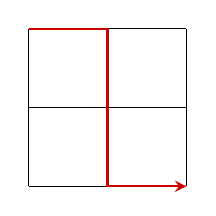
\begin{tikzpicture}
	\draw (0,0) grid (2, -2);
	\draw [->, >=stealth, thick, red!80!black] (0,0) -| (1, -2) -- (2, -2);
\end{tikzpicture}
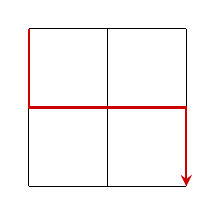
\begin{tikzpicture}
	\draw (0,0) grid (2, -2);
	\draw [->, >=stealth, thick, red!80!black] (0,0) |- (0, -1) -| (2, -2);
\end{tikzpicture}
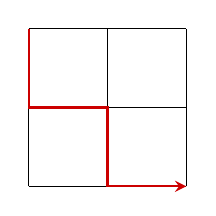
\begin{tikzpicture}
	\draw (0,0) grid (2, -2);
	\draw [->, >=stealth, thick, red!80!black] (0,0) |- (1, -1) |- (2, -2);
\end{tikzpicture}
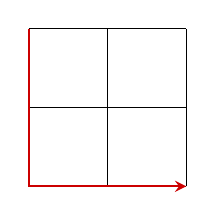
\begin{tikzpicture}
	\draw (0,0) grid (2, -2);
	\draw [->, >=stealth, thick, red!80!black] (0,0) |- (2, -2);
\end{tikzpicture}

How many such routes are there through a $20 \times 20$ grid?

\section{Solution}
\subsection{Combination}
\begin{align*}
	\binom nk = {}^nC_k & = \frac{n!}{(n-k)!k!}                                                           \\
	                    & = \frac{n \times (n - 1) \dots \times (k + 1)}{k \times (k - 1) \dots \times 1}
\end{align*}

\subsection{Dynamic Programming}
\begin{center}
	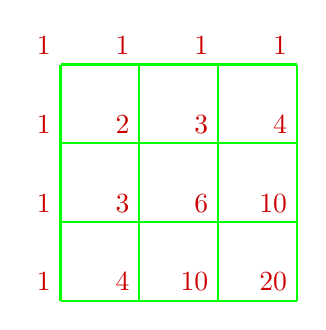
\begin{tikzpicture}
		\draw [green, thick](0,0) grid (3, -3);
		\node at (0,0)[above left, red!80!black]{1};
		\node at (1,0)[above left, red!80!black]{1};
		\node at (2,0)[above left, red!80!black]{1};
		\node at (3,0)[above left, red!80!black]{1};
		\node at (0,-1)[above left, red!80!black]{1};
		\node at (0,-2)[above left, red!80!black]{1};
		\node at (0,-3)[above left, red!80!black]{1};
		\node at (1,-1)[above left, red!80!black]{2};
		\node at (2,-1)[above left, red!80!black]{3};
		\node at (3,-1)[above left, red!80!black]{4};
		\node at (1,-2)[above left, red!80!black]{3};
		\node at (2,-2)[above left, red!80!black]{6};
		\node at (3,-2)[above left, red!80!black]{10};
		\node at (1,-3)[above left, red!80!black]{4};
		\node at (2,-3)[above left, red!80!black]{10};
		\node at (3,-3)[above left, red!80!black]{20};
	\end{tikzpicture}
\end{center}
